\onehalfspacing
\chapter*{Metodología}
Con el objetivo de desarrollar una plataforma que se ajuste al modelo de negocio  planteado por Ruta N, se asistió a unas sesiones de acompañamiento con el  laboratorio de creación que dispone la corporación; En estas sesiones se buscaba  plantear de manera clara la necesidad que busca solventar la plataforma, identificar el mercado objetivo y sus competencias, prototipado de la solución y por ultimo  aterrizar un modelo de negocio viable. \\

Las sesiones del laboratorio se distribuyeron en una sesión de 4 horas
semanal  durante cuatro semanas donde se utilizó una  metodología compuesta por conceptos  de design thinking (ver figura 1) y  metodología doble diamante (ver figura 2).


\begin{figure}[ht]
  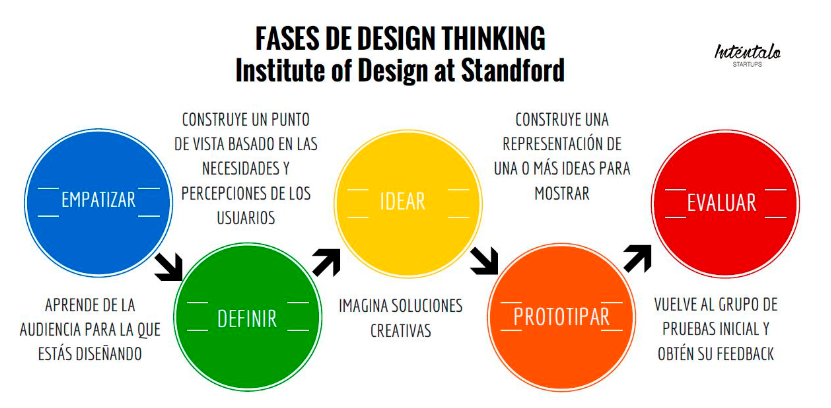
\includegraphics[width=\linewidth, center]{images/design_thinking.PNG}
  \caption{Proceso de la metodologia Design thinking. Tomado de \url{http://cursoparaemprendedoresuned.intentalo.es}}
  \label{fig:img1}
\end{figure}

\begin{figure}[]
  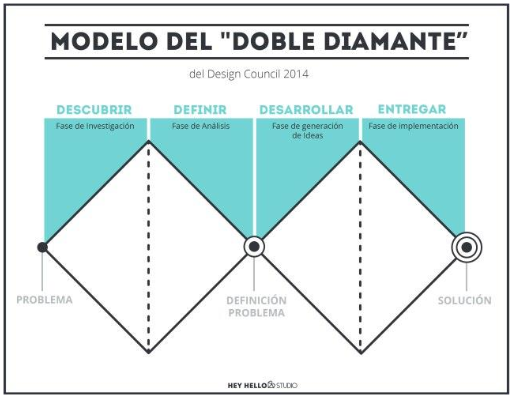
\includegraphics[scale=0.8, center]{images/doble_diamante.PNG}
  \caption{Proceso de la metodologia Doble diamante. Tomado de \url{https://i.pinimg.com}}
  \label{fig:img2}
\end{figure}


\begin{itemize}
    \item Primera sesión: Se aterrizó la idea del negocio con el fin de que los miembros del equipo manejaran la misma terminología y se centraran en un mismo objetivo, se identificaron posibles aspectos políticos , ambientales, sociales, tecnológicos, económicos y legales que pueden afectar el desarrollo o que hicieran inviable la idea de negocio, además, se detallaron los actores que interactuaran con la plataforma y su rol dentro de la misma. Esta sesión debió ser validada con un posible cliente esperando su nivel de aprobación y posibles recomendaciones o expectativas.
    \item  Segunda sesión: Se desglosó el objetivo principal de la plataforma en momentos clave que permitieran alcanzar un producto mínimo viable, se detallaron objetivos específicos del desarrollo y se especificaron las tácticas o metodologías y los instrumentos necesarios para llevar a cabo los objetivos. 
    \item Tercera sesión: Esta sesión se dedicó exclusivamente a la creación de prototipos de la plataforma con el fin de que fueran validados por algunos posibles clientes e identificar los puntos interesantes, ideas para incluir en futuros prototipos y críticas constructivas.
    \item Cuarta sesión: Esta sesión se destinó para planear el trabajo futuro y definir los pasos a seguir para cumplir con los objetivos del desarrollo, teniendo en cuenta tanto el desarrollo técnico como el de la marca, pruebas técnicas , financiamiento del proyecto, activación de la marca y mercado objetivo.
\end{itemize}

En cada una de las sesiones se llenaron formatos que permitieron sintetizar lo realizado y guías de validación las cuales fueron diligenciadas con los posibles clientes como \href{http://www.tecnnova.org/}{Tecnnova} \\

Luego del acompañamiento con el laboratorio de creación y el levantamiento de requisitos se procedió a diseñar la arquitectura de la plataforma en la cual se incluyen las tecnologías sobre las cuales se debe realizar el desarrollo.